\chapter{Động lực học Friedmann: vật chất, bức xạ và năng lượng chân không}

\lectureoverview{Động học của một vũ trụ đang giãn nở có thể được phát biểu trong một dòng: các khoảng cách vật lý tăng theo một hệ số tỉ lệ \(a(t)\). Vấn đề bây giờ là xác định hàm đó. Chúng ta sẽ khôi phục phương trình Friedmann cho không gian phẳng từ định luật bảo toàn năng lượng Newton, trước hết giải nó cho vật chất thông thường, rồi xem vì sao bức xạ và năng lượng chân không dẫn đến những lịch sử vũ trụ hoàn toàn khác nhau.}

\section{Hình học cần được giải thích}

Tại một thời điểm vũ trụ cố định, vũ trụ trên quy mô lớn có vẻ đồng nhất và đẳng hướng. Các thiên hà, cụm thiên hà và siêu cụm thiên hà chắc chắn là những cấu trúc có thật, nhưng ở các thang cỡ hàng trăm triệu hay hàng tỉ năm ánh sáng, sự phân bố của chúng trở nên đồng đều một cách đáng kinh ngạc. Tính đều đặn thực nghiệm này được gọi là nguyên lý vũ trụ học. Tên gọi ấy không biến nó thành một định lý; sức nặng của nguyên lý đến từ quan sát.

Có một dữ kiện thực nghiệm thứ hai. Trong độ chính xác hiện nay, các tam giác không gian lớn ứng xử như các tam giác Euclid. So sánh với việc đo đạc một sân bóng đá là hữu ích. Nếu những sợi dây căng chặt tạo thành các tam giác có tổng các góc bằng \(180^\circ\), thì ta chưa chứng minh được rằng Trái Đất là phẳng trên toàn cục. Ta đã chỉ ra rằng bán kính cong của Trái Đất lớn so với sân đó. Trắc địa vũ trụ có cùng dạng logic: không gian có thể có một bán kính cong rất lớn, nhưng trên miền quan sát được nó được xấp xỉ tốt là phẳng.

Hình học tham chiếu là không-thời gian Minkowski,
\begin{equation}
  d\tau^2=dt^2-\left(dx^2+dy^2+dz^2\right).
  \label{eq:l09-minkowski}
\end{equation}
Biểu thức trong ngoặc đơn đơn thuần là phần tử khoảng cách Euclid trong ba chiều. Trái lại, trong thuyết tương đối rộng, các hệ số của các vi phân tọa độ là các trường. Chúng có thể biến thiên theo vị trí và thời gian, và các hạng trộn cũng có thể xuất hiện. Các hệ số metric này là những đối tượng kế thừa trong tương đối tính của trường hấp dẫn Newton.

\begin{figure}[H]
  \centering
  \includegraphics[width=0.72\textwidth]{lecture_09_figure_01.png}
  \caption{Phần tử thời gian riêng Minkowski được viết ở đầu bài giảng. Khung hình nguồn tại 00:01:50.}
  \label{fig:l09-minkowski-board}
\end{figure}

Đối với một vũ trụ đang giãn nở phẳng theo không gian, tính đồng nhất và đẳng hướng chỉ để lại một hệ số tỉ lệ phụ thuộc thời gian:
\begin{equation}
  d\tau^2=dt^2-a^2(t)\left(dx^2+dy^2+dz^2\right).
  \label{eq:l09-flat-frw}
\end{equation}
Ta dùng đơn vị trong đó \(c=1\), nên thời gian và độ dài có cùng thứ nguyên. Có hai quy ước nhất quán. Có thể gán cho \(x,y,z\) thứ nguyên độ dài và lấy \(a\) không thứ nguyên, hoặc coi \(x,y,z\) là các nhãn không thứ nguyên và để \(a\) mang thứ nguyên độ dài. Bài giảng dùng quy ước thứ hai vì nó làm lộ rõ ý nghĩa vật lý của \(a(t)\).

\begin{figure}[H]
  \centering
  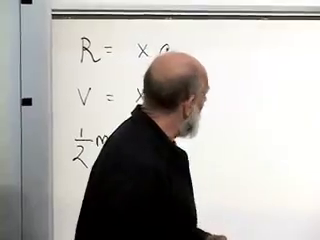
\includegraphics[width=0.72\textwidth]{lecture_09_figure_02.png}
  \caption{Metric phẳng đang giãn nở, với hệ số tỉ lệ nhân vào phần tử độ dài không gian Euclid. Khung hình nguồn tại 00:09:12.}
  \label{fig:l09-expanding-metric-board}
\end{figure}

Hãy tưởng tượng các tọa độ được vẽ trên một tấm cao su. Các dấu tọa độ vẫn gắn với tấm đó trong khi khoảng cách vật lý giữa chúng tăng lên. Vì thế, một hiệu tọa độ như "từ \(x=0\) đến \(x=1\)" chỉ là một cặp nhãn. Khoảng cách mà khoảng đó biểu diễn là \(a(t)\). Tìm phương trình chi phối hệ số tỉ lệ này là bài toán động lực học của bài giảng.

\section{Các hình học không gian kín, phẳng và mở}

Tính phẳng là một sự đơn giản hóa do quan sát, không phải là hệ quả của tính đồng nhất. Có ba hình học không gian vừa đồng nhất vừa đẳng hướng: độ cong dương, bằng 0 và âm. Để hiểu trường hợp dương, cần nói chính xác về số chiều.

Quỹ tích
\begin{equation}
  X_1^2+X_2^2=R^2
\end{equation}
là một đường tròn, hay mặt cầu một chiều \(S^1\). Phần trong đặc của nó là một đĩa, còn gọi là quả cầu hai chiều. Thêm một tọa độ nhúng nữa ta được
\begin{equation}
  X_1^2+X_2^2+X_3^2=R^2,
\end{equation}
mặt cầu hai chiều thông thường \(S^2\). Thêm một tọa độ nhúng thứ tư ta được
\begin{equation}
  X_1^2+X_2^2+X_3^2+X_4^2=R^2,
  \label{eq:l09-three-sphere}
\end{equation}
một mặt cầu ba chiều \(S^3\), bản thân nó là một không gian ba chiều. Ta không thể hình dung phép nhúng bốn chiều của nó, nhưng hình học nội tại không cần phép nhúng ấy để tồn tại.

\begin{figure}[H]
  \centering
  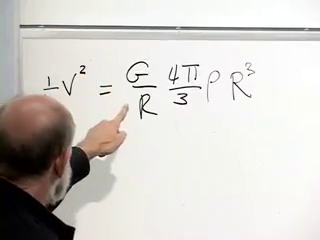
\includegraphics[width=0.72\textwidth]{lecture_09_figure_03.png}
  \caption{Phương trình nhúng dùng để giới thiệu mặt cầu ba chiều. Khung hình nguồn tại 00:16:40.}
  \label{fig:l09-three-sphere-board}
\end{figure}

Mọi điểm trên một mặt cầu lý tưởng đều tương đương về mặt hình học với mọi điểm khác, và mọi hướng tại một điểm đều tương đương. Vì thế, một mặt cầu vừa đồng nhất vừa đẳng hướng. Nếu bán kính của nó được nhân với \(a(t)\), toàn bộ không gian sẽ giãn ra hoặc co lại mà không chọn ra một tâm nào trên mặt cầu. Lần ngược một vũ trụ như vậy về quá khứ không đặt toàn bộ vật chất vào một vị trí đặc biệt nào trong một khoảng trống bên ngoài. Toàn bộ không gian trở nên nhỏ lại, nên mọi cặp điểm đều trở nên gần nhau. Vụ Nổ Lớn không phải là một vụ nổ từ một điểm của không gian.

Trên một mặt cầu có độ cong dương, các tam giác trắc địa có tổng góc lớn hơn \(180^\circ\). Các tam giác phẳng có tổng góc đúng bằng \(180^\circ\). Trong một hình học đồng nhất có độ cong âm, được biểu diễn không hoàn hảo bằng một mặt yên ngựa, tổng góc nhỏ hơn \(180^\circ\). Các phép kiểm tra nội tại này phân biệt ba trường hợp.

\begin{figure}[H]
  \centering
  \includegraphics[width=0.72\textwidth]{lecture_09_figure_07.png}
  \caption{Độ cong dương, bằng 0 và âm được phác họa qua các dạng tam giác đặc trưng của chúng. Khung hình nguồn tại 00:37:30.}
  \label{fig:l09-curvature-board}
\end{figure}

Một metric cục bộ phẳng hoàn toàn tự nó không chứng minh rằng không gian là vô hạn về tô pô. Các tô pô phẳng compact là khả dĩ về mặt toán học, mặc dù bài giảng dùng mô hình Euclid vô hạn đơn giản nhất.
\editorialnote{Bảo lưu về tô pô toàn cục này không cần đến cho bất kỳ động lực học cục bộ nào về sau.}

\section{Nhãn đồng chuyển động và định luật Hubble}

Bây giờ hãy trở lại tấm phẳng đang giãn nở và vẽ lên đó một lưới tọa độ. Trong tọa độ đồng chuyển động, lưới này giãn nở cùng với dòng vật chất quy mô lớn. Một thiên hà, hay chính xác hơn là một cụm thiên hà được làm trơn ở thang đủ thô, giữ một nhãn tọa độ xấp xỉ cố định mặc dù khoảng cách vật lý của nó tới một vật thể đồng chuyển động khác thay đổi.

\begin{figure}[H]
  \centering
  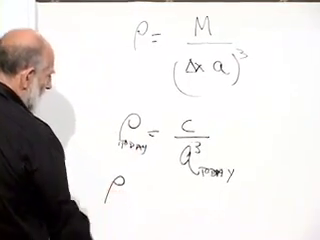
\includegraphics[width=0.72\textwidth]{lecture_09_figure_04.png}
  \caption{Một lưới tọa độ được mang theo bởi một tấm không gian đang giãn nở. Khung hình nguồn tại 00:22:20.}
  \label{fig:l09-comoving-grid-board}
\end{figure}

Đối với hai vật thể cách nhau dọc theo trục \(x\) bởi một khoảng đồng chuyển động cố định \(\Delta x\), khoảng cách vật lý của chúng là
\begin{equation}
  D(t)=a(t)\,\Delta x.
  \label{eq:l09-physical-distance}
\end{equation}
Lấy đạo hàm trong khi giữ \(\Delta x\) cố định, ta được
\begin{equation}
  v(t)=\dot a(t)\,\Delta x
      =\frac{\dot a(t)}{a(t)}D(t).
\end{equation}
Định nghĩa
\begin{equation}
  H(t)\equiv\frac{\dot a(t)}{a(t)},
  \label{eq:l09-hubble-parameter}
\end{equation}
ta thu được định luật Hubble,
\begin{equation}
  v=H(t)D.
  \label{eq:l09-hubble-law}
\end{equation}
Từ "hằng số" trong "hằng số Hubble" có nghĩa là không đổi theo không gian tại một thời điểm vũ trụ xác định. Nó không hàm ý tính không đổi trong suốt lịch sử vũ trụ.

\begin{figure}[H]
  \centering
  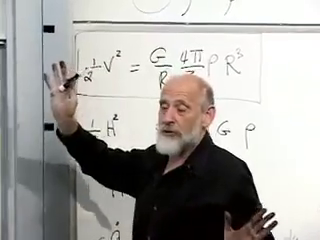
\includegraphics[width=0.72\textwidth]{lecture_09_figure_05.png}
  \caption{Phép suy ra trên bảng \(D=a\Delta x\),
  \(v=(\dot a/a)D=HD\). Khung hình nguồn tại 00:26:40.}
  \label{fig:l09-hubble-board}
\end{figure}

\begin{classroomqa}
\audiencequestion{Nếu một thiên hà xa được quan sát ở một thời điểm sớm hơn, liệu tham số Hubble suy ra cho nó có thật sự bằng giá trị được đo ở gần chúng ta ngày nay không?}
\lecturerresponse{Chỉ khi thời gian nhìn lùi nhỏ so với tuổi của vũ trụ. Ở các khoảng cách vừa phải, \(H(t)\) biến thiên đủ ít để một con số vẫn hữu ích. Ở các khoảng cách thật sự vũ trụ học, ta nhìn thấy những kỷ nguyên sớm hơn, và phải tính đến sự phụ thuộc theo thời gian của \(a\) và \(H\). Đó là một lý do khiến ta cần một phương trình động lực học cho hệ số tỉ lệ.}
\end{classroomqa}

\section{Tia null trong một hệ tọa độ đang giãn nở}

\begin{classroomqa}
\audiencequestion{Hệ số tỉ lệ có ảnh hưởng đến sự truyền ánh sáng giữa các thiên hà xa không?}
\lecturerresponse{Một tia sáng đi theo một quỹ đạo null, nên \(d\tau=0\). Đối với một tia chuyển động dọc theo trục \(x\) dương, \(dy=dz=0\), và metric giãn nở cho
\begin{align}
  0&=dt^2-a^2(t)dx^2,
  &dt&=a(t)dx,\notag\\
  &&\frac{dx}{dt}&=\frac{1}{a(t)}.
  \label{eq:l09-null-ray}
\end{align}
Vận tốc tọa độ giảm khi \(a(t)\) tăng, nhưng tốc độ ánh sáng vật lý cục bộ vẫn là \(c=1\). Một khoảng tọa độ cố định biểu diễn một khoảng cách vật lý ngày càng lớn.}
\end{classroomqa}

\begin{figure}[H]
  \centering
  \includegraphics[width=0.72\textwidth]{lecture_09_figure_06.png}
  \caption{Điều kiện null và \(dt=a(t)dx\) đối với sự truyền ánh sáng xuyên tâm. Khung hình nguồn tại 00:30:54.}
  \label{fig:l09-null-board}
\end{figure}

Người ta có thể chọn các tọa độ trong đó cùng một sự kiện này được diễn đạt như "ánh sáng chậm đi khi ở xa hơn", nhưng khi ấy các độ dài và đồng hồ lại nhận những mô tả tương ứng vụng về. Cách nói không gian giãn nở gọn hơn vì nó bảo toàn phát biểu cục bộ rằng mọi quan sát viên rơi tự do đều đo cùng một tốc độ ánh sáng.

\begin{classroomqa}
\audiencequestion{Có bằng chứng nào cho thấy sự truyền ánh sáng cục bộ và vật lý nguyên tử là như nhau trong các thiên hà xa không?}
\lecturerresponse{Chỉ những so sánh không thứ nguyên mới có ý nghĩa thao tác. Hãy chọn một kích thước nguyên tử làm đơn vị độ dài và một chu kỳ nguyên tử hoặc hạt nhân làm đơn vị thời gian, rồi hỏi ánh sáng cần bao nhiêu chu kỳ như vậy để đi qua độ dài đã chọn. Các quan sát quang phổ ủng hộ khẳng định rằng các tỉ số không thứ nguyên này là như nhau ở các vùng xa. Bằng chứng là gián tiếp, nhưng đó chính xác là kiểu so sánh dùng để kiểm tra tính đồng nhất của các định luật cục bộ.}
\end{classroomqa}

Khi vũ trụ quan sát được cực kỳ nhỏ, ánh sáng có thể băng qua một miền vật lý cho trước rất nhanh nếu đo bằng đơn vị thời gian ánh sáng băng qua tương ứng. Điều này không có nghĩa là \(c\) đã khác. Nó có nghĩa là chính miền đó khi ấy nhỏ.

\section{Một hình cầu Newton bên trong vũ trụ}

Bây giờ ta chuyển từ động học sang động lực học. Hãy đặt mình tại gốc tọa độ và vẽ một hình cầu đủ lớn để chứa nhiều thiên hà và cụm thiên hà. Chọn một thiên hà trên biên của nó. Trong một vũ trụ đồng nhất, phân bố khối lượng là đối xứng cầu quanh ta, và định lý vỏ cầu của Newton cho hai sự kiện then chốt:
\begin{enumerate}
  \item mọi vật chất được phân bố cầu ở ngoài bán kính đã chọn tác dụng lực Newton tổng cộng bằng 0 lên thiên hà ở biên;
  \item mọi vật chất ở bên trong hình cầu tác dụng, đối với chuyển động theo phương bán kính này, như thể nó tập trung tại tâm.
\end{enumerate}
Ta dùng một hệ quy chiếu trong đó ta đứng yên, nên các vận tốc và gia tốc trong lập luận sau đây được đo tương đối so với ta.

\begin{figure}[H]
  \centering
  \includegraphics[width=0.72\textwidth]{lecture_09_figure_08.png}
  \caption{Cấu dựng theo định lý vỏ cầu: ta ở tâm và một thiên hà thử trên biên của một hình cầu đồng nhất lớn. Khung hình nguồn tại 00:41:10.}
  \label{fig:l09-shell-board}
\end{figure}

\begin{figure}[H]
  \centering
  \begin{tikzpicture}[scale=0.92,>=Latex]
    \draw[thick] (0,0) circle (2.35);
    \fill (0,0) circle (2pt) node[below left] {us};
    \fill (2.35,0) circle (2.2pt) node[right] {test galaxy \(m\)};
    \draw[->,thick,blue!65!black] (0.18,0) -- (2.15,0)
      node[midway,above] {\(R=a(t)x\)};
    \draw[->,thick,red!65!black] (2.35,0.12) -- (3.25,0.12)
      node[midway,above] {\(v=\dot a(t)x\)};
    \node[align=center,text width=7cm] at (0,-2.85)
      {outside shells cancel;\\enclosed mass acts at the center};
  \end{tikzpicture}
  \caption{Phục dựng gọn của cấu dựng Newton.}
  \label{fig:l09-shell-clean}
\end{figure}

Nếu thiên hà có tọa độ đồng chuyển động cố định \(x\), thì bán kính vật lý và vận tốc của nó là
\begin{equation}
  R(t)=x a(t),
  \qquad
  v(t)=x\dot a(t)=H(t)R(t).
  \label{eq:l09-radius-velocity}
\end{equation}
Gọi \(M\) là khối lượng bao trong hình cầu và \(m\) là khối lượng của thiên hà thử. Năng lượng Newton là
\begin{equation}
  E=\frac12 m v^2-\frac{GMm}{R}.
  \label{eq:l09-newtonian-energy}
\end{equation}

\begin{figure}[H]
  \centering
  \includegraphics[width=0.72\textwidth]{lecture_09_figure_09.png}
  \caption{Toàn bộ chuỗi suy ra trên bảng \(R=xa\), \(v=x\dot a\), và phương trình năng lượng Newton được chuyên biệt hóa cho \(E=0\). Khung hình nguồn tại 00:48:40.}
  \label{fig:l09-energy-board}
\end{figure}

Năng lượng có thể dương, bằng 0 hoặc âm. Hãy bắt đầu ở ranh giới giữa thoát ly và co sụp trở lại, \(E=0\), khi đó
\begin{equation}
  \frac12 v^2=\frac{GM}{R}.
  \label{eq:l09-zero-energy}
\end{equation}

\begin{classroomqa}
\audiencequestion{Tổng năng lượng bằng 0 có nghĩa gì đối với thiên hà đang lùi ra xa?}
\lecturerresponse{Đó chính xác là trường hợp vận tốc thoát. Năng lượng dương nghĩa là chuyển động vượt vận tốc thoát; năng lượng âm nghĩa là chuyển động dưới vận tốc thoát và, trong bức tranh Newton chỉ gồm vật chất, là cuối cùng quay trở lại. Ta bắt đầu ở ranh giới giữa các khả năng đó và sẽ quay lại các dấu kia sau khi suy ra phương trình phẳng.}
\end{classroomqa}

\begin{classroomqa}
\audiencequestion{Liệu \(M\), khối lượng bao trong, có biến thiên khi hình cầu giãn nở không?}
\lecturerresponse{Không. Hình cầu là đồng chuyển động, nên vẫn chính những hạt ấy ở bên trong nó. Thể tích vật lý của nó tăng lên và mật độ của nó giảm xuống, nhưng tổng khối lượng bao trong vẫn giữ cố định. Sự phân biệt này giữa \(M\) và \(\rho(t)\) là thiết yếu.}
\end{classroomqa}

Với mật độ đồng nhất \(\rho(t)\),
\begin{equation}
  M=\frac{4\pi}{3}\rho(t)R^3.
  \label{eq:l09-enclosed-mass}
\end{equation}
Thay vào \eqref{eq:l09-zero-energy} ta được
\begin{equation}
  \frac12 v^2
  =\frac{G}{R}\left(\frac{4\pi}{3}\rho R^3\right).
  \label{eq:l09-enclosed-energy}
\end{equation}

\begin{figure}[H]
  \centering
  \includegraphics[width=0.72\textwidth]{lecture_09_figure_10.png}
  \caption{Phép thay thế bằng khối lượng chứa bên trong trong phương trình năng lượng bằng 0.
  Khung hình nguồn tại 00:54:16.060.}
  \label{fig:l09-enclosed-mass-board}
\end{figure}

Dùng \(v=HR\), ta được
\begin{align}
  \frac12 H^2R^2
    &=\frac{4\pi G}{3}\rho R^2,\\
  H^2
    &=\frac{8\pi G}{3}\rho.
\end{align}
Do đó, định luật giãn nở năng lượng bằng 0, phẳng theo không gian là
\begin{equation}
  \boxed{\left(\frac{\dot a}{a}\right)^2
  =\frac{8\pi G}{3}\rho(t)}.
  \label{eq:l09-flat-friedmann}
\end{equation}
Sự triệt tiêu của \(R^2\) không phải là ngẫu nhiên. Một vũ trụ đồng nhất phải
cho cùng \(H(t)\) bất kể thiên hà đồng chuyển động nào được chọn làm vật thử.

\begin{figure}[H]
  \centering
  \includegraphics[width=0.72\textwidth]{lecture_09_figure_11.png}
  \caption{Sự triệt tiêu của bán kính và hệ thức Friedmann phẳng thu được trên bảng.
  Khung hình nguồn tại 00:57:30.}
  \label{fig:l09-friedmann-board}
\end{figure}

\begin{classroomqa}
\audiencequestion{Có bằng chứng nào cho hệ thức năng lượng bằng 0 không?}
\lecturerresponse{Cả hai vế đều có thể được suy ra từ quan sát: \(H\) từ
dữ liệu lùi xa và \(\rho\) bằng cách tính đến sao, khí, vật chất tối và
năng lượng chân không. Phép so sánh vào thời điểm bài giảng cho thấy hai vế
phù hợp với nhau ở mức chính xác cỡ phần trăm. Điều bảo lưu này rất quan
trọng: phải bao gồm mọi dạng năng lượng, và phần thảo luận sau về năng lượng
chân không làm thay đổi cách diễn giải ngây thơ theo vận tốc thoát.}
\end{classroomqa}

Trong hệ đơn vị \(c=1\), mật độ khối lượng và mật độ năng lượng có cùng đơn vị. Ký
hiệu \(\rho\) vì thế sẽ chỉ tổng mật độ năng lượng thích hợp với thành phần đang
được bàn tới.

\section{Vật chất thông thường và quy luật hai phần ba}

Phương trình \eqref{eq:l09-flat-friedmann} chưa khép kín cho đến khi ta biết
\(\rho(t)\) biến thiên như thế nào. Trước hết hãy lấp đầy một hộp chữ nhật đồng
chuyển động bằng các hạt chuyển động chậm, phi tương đối tính. Các kích thước
tọa độ của nó là cố định, còn thể tích vật lý tăng theo
\begin{equation}
  V(t)=a^3(t)\,\Delta x\,\Delta y\,\Delta z.
\end{equation}
Số hạt và khối lượng nghỉ trong hộp giữ nguyên, nên
\begin{equation}
  \rho_{\mathrm m}(t)=\frac{C_{\mathrm m}}{a^3(t)}.
  \label{eq:l09-matter-dilution}
\end{equation}
Chuẩn hóa theo thời điểm hiện tại \(t_0\),
\begin{equation}
  \frac{\rho_{\mathrm m}(t)}{\rho_{\mathrm m,0}}
  =\left(\frac{a_0}{a(t)}\right)^3.
  \label{eq:l09-matter-normalized}
\end{equation}

\begin{figure}[H]
  \centering
  \includegraphics[width=0.72\textwidth]{lecture_09_figure_12.png}
  \caption{Mật độ vật chất, sự pha loãng \(a^{-3}\) của nó và chuẩn hóa
  ở thời điểm hiện nay. Khung hình nguồn tại 01:04:47.940.}
  \label{fig:l09-density-board}
\end{figure}

\begin{classroomqa}
\audiencequestion{Mật độ năng lượng hiện nay của vũ trụ xấp xỉ là bao nhiêu,
và chỉ riêng các nguyên tử thông thường có thể cung cấp nó không?}
\lecturerresponse{Việc đếm vật chất baryon nhìn thấy được chỉ cho một phần
câu trả lời. Vật chất tối và năng lượng tối cũng phải được biểu diễn dưới dạng
khối lượng-năng lượng tương đương. Bài giảng nêu một thang xấp xỉ trải từ một
nguyên tử đến vài chục tương đương khối lượng hydro trên mỗi mét khối, nhấn
mạnh bậc độ lớn hơn là một kiểm kê chính xác.}
\end{classroomqa}

Thế \eqref{eq:l09-matter-dilution} vào
\eqref{eq:l09-flat-friedmann} và gộp mọi thừa số không phụ thuộc thời gian vào một hằng số
dương \(C\):
\begin{equation}
  \left(\frac{\dot a}{a}\right)^2=\frac{C}{a^3},
  \qquad
  \dot a^2=\frac{C}{a}.
  \label{eq:l09-matter-ode}
\end{equation}
Có hai cách minh bạch để giải nó. Một phép thử dạng lũy thừa
\(a=K t^p\) đòi hỏi
\begin{equation}
  p-1=-\frac{p}{2},
  \qquad p=\frac23.
\end{equation}
Tương đương, chọn nhánh căn bậc hai ứng với giãn nở và tích phân:
\begin{equation}
  a^{1/2}\frac{da}{dt}=\sqrt C,
  \qquad
  \int a^{1/2}da=\sqrt C\int dt,
\end{equation}
nên, sau khi chọn gốc thời gian tại Big Bang,
\begin{equation}
  a^{3/2}\propto t,
  \qquad
  \boxed{a(t)\propto t^{2/3}}.
  \label{eq:l09-matter-solution}
\end{equation}
Trong phép suy dẫn trực tiếp, có lúc tạm thời làm mất một thừa số khi ghép hệ
số, rồi quay lại phép tích phân và kiểm tra số mũ. Ghi chú giữ lại phép kiểm
tra nhưng chỉ trình bày đại số đã hiệu chỉnh.

\begin{figure}[H]
  \centering
  \includegraphics[width=0.72\textwidth]{lecture_09_figure_13.png}
  \caption{Phép thử dạng lũy thừa và số mũ được đóng khung \(p=2/3\). Khung hình nguồn
  tại 01:13:05.}
  \label{fig:l09-matter-solution-board}
\end{figure}

Lấy đạo hàm của nghiệm cho
\begin{equation}
  H(t)=\frac{\dot a}{a}=\frac{2}{3t}.
  \label{eq:l09-matter-hubble}
\end{equation}
Tham số Hubble trong quá khứ lớn hơn. Do đó, khi nhìn đủ xa để thấy thời gian
nhìn lùi đáng kể, ta không nên kéo dài quan hệ tuyến tính cục bộ mà vẫn giữ
nguyên \(H_0\) hiện nay.

\begin{figure}[H]
  \centering
  \includegraphics[width=0.72\textwidth]{lecture_09_figure_14.png}
  \caption{Lấy \(\dot a/a\) của \(a\propto t^{2/3}\) cho
  \(H=2/(3t)\). Khung hình nguồn tại 01:20:42.}
  \label{fig:l09-hubble-time-board}
\end{figure}

\section{Dấu của năng lượng và độ cong không gian}

Lập luận kiểu Newton đã đưa ta đi qua trường hợp phẳng có năng lượng bằng 0. Thuyết
 tương đối rộng bổ sung một sự kiện không thể thu được chỉ từ định lý vỏ cầu:
dấu của năng lượng riêng kiểu Newton tương ứng với dấu của độ cong không
gian.
\begin{center}
\begin{tabular}{@{}>{\raggedright\arraybackslash}p{0.20\linewidth}
                    >{\raggedright\arraybackslash}p{0.29\linewidth}
                    >{\raggedright\arraybackslash}p{0.37\linewidth}@{}}
  \toprule
  Tổng năng lượng & Độ cong không gian & Số phận khi chỉ có vật chất \\
  \midrule
  dương & âm (mở) & giãn nở mãi mãi \\
  bằng 0 & bằng 0 (phẳng) & tiệm cận ngưỡng thoát \\
  âm & dương (đóng) & giãn nở, quay đầu, tái co sụp \\
  \bottomrule
\end{tabular}
\end{center}
Cột cuối giả sử không có năng lượng chân không. Trong phép tương tự vật phóng, năng lượng
dương nghĩa là trên vận tốc thoát, bằng 0 nghĩa là đúng bằng vận tốc thoát,
và âm nghĩa là dưới vận tốc thoát. Các phương trình Einstein đồng nhất ba
trường hợp này lần lượt với hình học không gian mở, phẳng và đóng.

\section{Photon và quy luật một phần hai}

Quy luật vật chất \(\rho\propto a^{-3}\) giả sử rằng năng lượng của mỗi hạt
xấp xỉ cố định trong khi mật độ số giảm xuống. Photon vi phạm giả định đó.
Đối với một photon,
\begin{equation}
  E=h\nu=\frac{hc}{\lambda}.
\end{equation}
Sự giãn nở làm bước sóng của nó dãn ra tỉ lệ với thừa số tỉ lệ,
\begin{equation}
  \lambda\propto a,
  \qquad E\propto a^{-1}.
\end{equation}
Mật độ số photon vẫn giảm như \(a^{-3}\), và năng lượng của mỗi photon đóng
góp thêm một thừa số \(a^{-1}\). Vì vậy
\begin{equation}
  \boxed{\rho_{\mathrm r}(t)\propto a^{-4}(t)}.
  \label{eq:l09-radiation-dilution}
\end{equation}

Phép tương tự dây đàn guitar nắm bắt bức tranh vật lý. Gảy một dây rồi kéo
dài phần đang dao động của nó: bước sóng dài ra và cao độ hạ xuống. Một mode
photon trong một hộp đồng chuyển động đang giãn nở cũng hành xử tương tự. Nếu
chạy ngược bức tranh, sự nén lại làm bước sóng ngắn đi và năng lượng photon
tăng lên.

\begin{figure}[H]
  \centering
  \includegraphics[width=0.72\textwidth]{lecture_09_figure_15.png}
  \caption{Hệ thức mật độ vật chất được mở rộng trên bảng thành
  quy luật tỉ lệ của bức xạ \(\rho_{\mathrm r}\propto a^{-4}\). Khung hình nguồn tại 01:29:20.}
  \label{fig:l09-radiation-board}
\end{figure}

Dùng \(\rho_{\mathrm r}\propto a^{-4}\) trong phương trình Friedmann phẳng, ta được
\begin{equation}
  \left(\frac{\dot a}{a}\right)^2=\frac{C_{\mathrm r}}{a^4},
  \qquad
  \dot a\propto a^{-1},
\end{equation}
và do đó
\begin{equation}
  \boxed{a(t)\propto t^{1/2}}.
  \label{eq:l09-radiation-solution}
\end{equation}
Nó tăng chậm hơn \(t^{2/3}\). Đi đủ xa về quá khứ, bức xạ tất phải trội hơn vật
chất thông thường vì \(a^{-4}\) tăng nhanh hơn \(a^{-3}\) khi \(a\) giảm.
Bài giảng đặt thời điểm chuyển tiếp vật chất-bức xạ vào khoảng khi thừa số tỉ
lệ nhỏ hơn hiện nay chừng một nghìn lần. Trước mốc chuyển tiếp đó, vũ trụ bị
bức xạ chi phối; sau đó, trong một khoảng dài, nó bị vật chất chi phối.

\section{Năng lượng chân không và giãn nở hàm mũ}

Năng lượng chân không có hành vi tỉ lệ hóa ngược lại. Mật độ của nó là một
thuộc tính của không gian trống và không bị pha loãng khi vũ trụ giãn nở:
\begin{equation}
  \rho_\Lambda=\text{constant}.
  \label{eq:l09-vacuum-density}
\end{equation}
Vật chất thông thường và bức xạ trở nên đậm đặc hơn khi đi về quá khứ, còn hạng
này thì không. Vì thế nó kém quan trọng hơn trong vũ trụ sơ khai và trở nên
quan trọng hơn khi các thành phần khác bị pha loãng. Bài giảng dùng ước lượng
đương thời rằng năng lượng chân không chiếm khoảng \(70\%\) mật độ năng lượng
vũ trụ hiện nay.

Với \(\rho_\Lambda\) không đổi, phương trình \eqref{eq:l09-flat-friedmann} cho một
tốc độ giãn nở không đổi
\begin{equation}
  H_\Lambda=\sqrt{\frac{8\pi G}{3}\rho_\Lambda},
  \qquad
  \frac{\dot a}{a}=H_\Lambda.
\end{equation}
Do đó
\begin{equation}
  \boxed{a(t)=a(t_i)e^{H_\Lambda(t-t_i)}}.
  \label{eq:l09-vacuum-solution}
\end{equation}

\begin{figure}[H]
  \centering
  \includegraphics[width=0.72\textwidth]{lecture_09_figure_16.png}
  \caption{Phương trình mật độ không đổi dẫn đến giãn nở hàm mũ.
  Khung hình nguồn tại 01:35:48.}
  \label{fig:l09-vacuum-board}
\end{figure}

Ở thang quan sát được nêu trong bài giảng, vũ trụ tăng gấp đôi kích thước tuyến tính trong khoảng chừng mười đến mười hai tỷ năm. Nguồn gốc của mật độ chân không nhỏ nhưng khác không này vẫn chưa được giải thích; sự tồn tại của nó cùng ảnh hưởng của nó đối với sự giãn nở là những dữ kiện thực nghiệm.

\begin{classroomqa}
\audiencequestion{Trong phần bàn luận này, năng lượng chân không có phải chính là năng lượng tối không?}
\lecturerresponse{Có. Ở đây “năng lượng tối” chỉ một mật độ năng lượng chân
không không đổi, tương đương với một hằng số vũ trụ học. Có thể hình dung
những mô hình năng lượng tối tổng quát hơn, phụ thuộc thời gian, nhưng chúng
không thuộc phép tính của bài giảng này.}
\end{classroomqa}

\section{Vũ trụ giãn nở làm dịch đỏ ánh sáng như thế nào}

\begin{classroomqa}
\audiencequestion{Làm sao photon có thể biết rằng ta đã chọn các tọa độ đồng
chuyển động đang giãn nở và vì thế làm giảm năng lượng của chúng?}
\lecturerresponse{Chúng không phản ứng với các nhãn của ta. Chúng lan truyền
trong một hình học mà các khoảng cách vật lý thay đổi. Một đoàn sóng chiếm
một vùng có kích thước vật lý tăng gấp đôi sẽ có bước sóng tăng gấp đôi. Các
tọa độ đồng chuyển động chỉ mô tả sự kéo giãn này một cách gọn gàng; chúng
không gây ra nó.}
\end{classroomqa}

\begin{classroomqa}
\audiencequestion{Các photon nền đến với ta ngày nay xuất phát từ đâu?}
\lecturerresponse{Nhìn càng xa nghĩa là nhìn càng sớm. Rồi đến lúc ta thấy
thời kỳ mà vật chất vũ trụ là một plasma ion hóa, mờ đục vì photon tán xạ lặp
đi lặp lại trên các hạt mang điện tự do. Biên mà từ đó photon lần cuối có thể
truyền tự do đến ta hiện ra như một mặt cầu bao quanh người quan sát: bề mặt
tán xạ cuối cùng.}
\end{classroomqa}

\begin{figure}[H]
  \centering
  \includegraphics[width=0.72\textwidth]{lecture_09_figure_17.png}
  \caption{Phác họa lấy người quan sát làm tâm của bề mặt tán xạ cuối cùng và
  các lớp vỏ ở xa dần. Khung hình nguồn tại 01:42:05.}
  \label{fig:l09-last-scattering-board}
\end{figure}

\begin{figure}[H]
  \centering
  \begin{tikzpicture}[scale=0.9,>=Latex]
    \fill (0,0) circle (2pt) node[below] {observer};
    \draw[thick,orange!70!black] (0,0) circle (2.55);
    \node[orange!70!black,align=center] at (0,3.05)
      {surface of last scattering};
    \foreach \a in {25,75,145,210,285,335}{
      \draw[->,blue!60!black] ({2.55*cos(\a)},{2.55*sin(\a)}) --
        ({1.7*cos(\a)},{1.7*sin(\a)});
    }
    \draw[decorate,decoration={snake,amplitude=1.5pt,segment length=7pt},
      red!65!black,thick,->] (-2.5,0) -- (-0.15,0);
    \node[red!65!black,below] at (-1.35,-0.15)
      {redshifted photon};
  \end{tikzpicture}
  \caption{Bản dựng lại rõ ràng của bức tranh tán xạ cuối cùng.}
  \label{fig:l09-last-scattering-clean}
\end{figure}

Bức xạ được phát ra với phổ đặc trưng của một plasma nóng và đến với ta với
bước sóng dài hơn xấp xỉ một nghìn lần. Theo ngôn ngữ Doppler của bài giảng,
bề mặt phát xạ ở xa lùi ra nhanh và bức xạ của nó bị dịch đỏ mạnh. Theo ngôn
ngữ hình học, sóng bị kéo giãn trong quá trình lan truyền. Cả hai cách nhìn
đều mã hóa cùng một hệ thức,
\begin{equation}
  1+z=\frac{\lambda_0}{\lambda_{\mathrm{em}}}
      =\frac{a_0}{a_{\mathrm{em}}}.
  \label{eq:l09-cosmological-redshift}
\end{equation}
\editorialnote{Phương trình \eqref{eq:l09-cosmological-redshift} là dạng định lượng chuẩn của các mô tả
kéo giãn và Doppler trong bài giảng.}

Ở một thời điểm quan sát sớm hơn, mặt cầu tán xạ cuối cùng trong bức tranh
tương ứng sẽ ở gần hơn, và các photon nền quan sát được sẽ bị dịch đỏ ít hơn
nên giàu năng lượng hơn. Khi thời gian vũ trụ trôi đi, các photon đi tới một
người quan sát đồng chuyển động từ plasma sơ khai ấy có bước sóng ngày càng
dài hơn.

\section{Năng lượng của một photon bị dịch đỏ đi đâu?}

\begin{classroomqa}
\audiencequestion{Một photon được phát ra với năng lượng \(h\nu_{\mathrm{em}}\) và
đến nơi trong trạng thái bị dịch đỏ với năng lượng nhỏ hơn. Điều gì đã xảy ra
với phần chênh lệch?}
\lecturerresponse{Phép suy dẫn kiểu Newton khởi đầu từ một phương trình năng
lượng. Dạng vũ trụ học của nó liên hệ tốc độ giãn nở với mật độ năng lượng vật
chất, nên không thể xem năng lượng của vật chất và sự giãn nở như những sổ cái
bảo toàn tách biệt. Bài giảng mô tả phần năng lượng photon bị mất là đi vào
phần hạch toán động năng của sự giãn nở. Một pít-tông chứa đầy bức xạ làm phép
tương tự trở nên cụ thể: áp suất bức xạ đẩy pít-tông ra ngoài, bước sóng photon
tăng lên, và phần năng lượng bị mất của chúng trở thành công cơ học và động năng
của pít-tông.}
\end{classroomqa}

\begin{figure}[H]
  \centering
  \includegraphics[width=0.72\textwidth]{lecture_09_figure_18.png}
  \caption{Trên bảng, phương trình năng lượng kiểu Newton được đóng khung nằm phía trên
  phương trình Friedmann tương ứng. Khung hình nguồn tại 01:44:42.}
  \label{fig:l09-energy-bookkeeping-board}
\end{figure}

\begin{classroomqa}
\audiencequestion{Điều gì ghép nối năng lượng bức xạ với sự giãn nở?}
\lecturerresponse{Áp suất. Trong một xi lanh với pít-tông di động, photon
truyền động lượng cho thành. Khi pít-tông chuyển động, bức xạ thực hiện công;
bước sóng của nó tăng lên và năng lượng của nó giảm xuống. Vũ trụ đồng nhất
đang giãn nở không có một pít-tông ngoài theo nghĩa đen, nhưng phép tương tự
\(p\,dV\) giải thích vì sao mật độ năng lượng của bức xạ giảm nhanh hơn so với
chỉ do sự pha loãng số lượng.}
\end{classroomqa}

\begin{figure}[H]
  \centering
  \includegraphics[width=0.72\textwidth]{lecture_09_figure_19.png}
  \caption{Pít-tông di động chứa photon được dùng để hình dung công áp suất.
  Khung hình nguồn tại 01:46:40.}
  \label{fig:l09-piston-board}
\end{figure}

\begin{figure}[H]
  \centering
  \begin{tikzpicture}[scale=0.92,>=Latex]
    \draw[thick] (0,0) rectangle (5.3,2.6);
    \draw[very thick] (4.25,0) -- (4.25,2.6);
    \draw[very thick] (4.25,1.3) -- (5.25,1.3);
    \draw[->,thick,red!65!black] (5.25,1.3) -- (6.2,1.3)
      node[right] {moving piston};
    \foreach \y in {0.55,1.3,2.05}{
      \draw[decorate,decoration={snake,amplitude=1.4pt,segment length=6pt},
        blue!65!black,->] (0.35,\y) -- (3.9,\y);
    }
    \node at (2.15,-0.45) {radiation does \(p\,dV\) work};
  \end{tikzpicture}
  \caption{Bản dựng lại rõ ràng của phép tương tự bức xạ–pít-tông.}
  \label{fig:l09-piston-clean}
\end{figure}

Năng lượng trong thuyết tương đối rộng đòi hỏi phải cẩn trọng. Trong một không-thời gian giãn nở tổng quát, không nhất thiết tồn tại một năng lượng toàn cục được bảo toàn duy nhất tương tự như năng lượng của một hệ Newton cô lập. Sự bảo toàn cục bộ năng lượng-động lượng vẫn đúng, và đối với một lưu chất đồng nhất, nó cho phương trình liên tục
\begin{equation}
  \dot\rho+3H(\rho+p)=0,
  \label{eq:l09-continuity}
\end{equation}
phương trình này chứa hạng công do áp suất đứng sau các định luật tỉ lệ của vật chất và bức xạ.\editorialnote{Phương trình \eqref{eq:l09-continuity} là phát biểu cục bộ chính xác của thuyết tương đối rộng làm cơ sở cho phép loại suy hạch toán năng lượng có chủ ý theo kiểu Newton trong bài giảng.}

Năng lượng chân không làm cho vấn đề ấy trở nên đặc biệt sắc nét. Vì mật độ của nó giữ không đổi trong khi thể tích tăng, tổng năng lượng chân không trong một vùng đồng chuyển động tăng lên. Áp suất âm của nó là một phần của nguồn hấp dẫn và thúc đẩy sự giãn nở gia tốc. Vì vậy, không nên đòi hỏi khái niệm ngây thơ về "năng lượng vật chất trong một hộp đồng chuyển động" phải được bảo toàn riêng biệt mà không tính cả hình học và công do áp suất.

\section{Vì sao có thể bỏ hệ số tỉ lệ khỏi hạng thời gian}

\begin{classroomqa}
\audiencequestion{Vì sao hệ số tỉ lệ nhân với phần không gian của metric mà không nhân với phần thời gian?}
\lecturerresponse{Đó là do cách chọn tọa độ thời gian. Giả sử ta bắt đầu với tọa độ thời gian bảo giác \(t\), trong đó
\begin{equation}
  d\tau^2=A^2(t)\left(dt^2-dx^2\right).
\end{equation}
Định nghĩa một thời gian vũ trụ mới \(T\) bởi
\begin{equation}
  dT=A(t)\,dt.
\end{equation}
Khi đó
\begin{equation}
  d\tau^2=dT^2-A^2\bigl(t(T)\bigr)dx^2.
\end{equation}
Hệ số chung đứng trước vi phân thời gian đã biến mất, trong khi hệ số tỉ lệ vật lý vẫn còn ở hạng không gian.}
\end{classroomqa}

\begin{figure}[H]
  \centering
  \includegraphics[width=0.72\textwidth]{lecture_09_figure_20.png}
  \caption{Phép tái định nghĩa thời gian \(dT=A(t)dt\) chuyển từ thời gian bảo giác sang thời gian vũ trụ. Khung hình gốc tại 01:51:05.}
  \label{fig:l09-time-reparam-board}
\end{figure}

\section{Độ cong, năng lượng chân không và số phận vũ trụ}

\begin{classroomqa}
\audiencequestion{Nếu vũ trụ có độ cong dương, liệu chúng ta đã phải thấy các thiên hà đang tiến lại gần chúng ta chưa?}
\lecturerresponse{Không nhất thiết. Một vật được phóng đi với vận tốc nhỏ hơn vận tốc thoát thì ban đầu sẽ đi ra xa, đạt tới một điểm ngoặt, và chỉ về sau mới rơi trở lại. Chúng ta quan sát vũ trụ trong một pha đang giãn nở. Nếu không có năng lượng chân không, một vũ trụ vật chất có độ cong dương cuối cùng sẽ co sụp trở lại. Một năng lượng chân không dương đủ lớn ngăn sự quay đầu đó, và giá trị quan sát được dường như đủ lớn để làm cho sự giãn nở về lâu dài diễn ra theo hàm mũ, bất kể một độ cong không gian nhỏ.}
\end{classroomqa}

Tương lai hàm mũ ấy không phải là một thiên đường về năng lượng. Các ngôi sao rốt cuộc sẽ cháy hết, mật độ vật chất và bức xạ giảm theo hàm mũ, và các vùng xa xôi vượt ra ngoài liên hệ nhân quả. Năng lượng chân không vẫn còn, trong khi các cấu trúc thông thường trở nên ngày càng lạnh hơn và loãng hơn.

\begin{classroomqa}
\audiencequestion{Nhìn xa hơn vào quá khứ, có nhiều photon hơn các hạt vật chất thông thường không?}
\lecturerresponse{Tỉ số số lượng photon trên baryon đã là khổng lồ, xấp xỉ \(10^{10}\) photon trên mỗi baryon theo ước tính của bài giảng, và cả hai số lượng trong một thể tích đồng chuyển động đều gần như giữ nguyên. Điều chủ yếu thay đổi khi nhìn ngược về quá khứ là năng lượng trên mỗi photon. Năng lượng photon tăng theo \(a^{-1}\), còn khối lượng nghỉ của vật chất phi tương đối tính thì không tăng như vậy. Vì vậy, bức xạ chi phối mật độ năng lượng ở các thời điểm sớm mặc dù bản thân tỉ số số lượng ấy không nhất thiết phải thay đổi.}
\end{classroomqa}

Bài học cốt lõi là chỉ riêng hình học không quyết định lịch sử vũ trụ. Phương trình Friedmann trong trường hợp phẳng cho quan hệ giữa sự giãn nở và mật độ năng lượng, nhưng thành phần của vũ trụ quyết định sự phụ thuộc theo thời gian. Vật chất phi tương đối tính cho \(a\propto t^{2/3}\), bức xạ cho \(a\propto t^{1/2}\), còn năng lượng chân không không đổi cho sự giãn nở hàm mũ. Ba quy luật đó định hình các kỷ nguyên kế tiếp nhau của vũ trụ và giải thích vì sao cùng một hệ số tỉ lệ chi phối các khoảng cách, các độ dịch đỏ và tham số Hubble đang thay đổi.